\section{Internal Combustion Engine Simulator}
%
ICESym es un simulador de motores de combustión interna que  utiliza modelos 0D
para la cámara de combustión y 1D para el flujo a través del sistema de
intercambio de gases.
%
Esta combinación permite evaluar la \emph{performance} de un motor a un costo
computacional relativamente bajo; además la implementación de entrada y salida
de datos facilita utilizar el simulador como una \emph{caja negra}.
%
Esta característica permite incluir al simulador en un \emph{script} como una
función, a la cual se le otorga un conjunto de parámetros de entrada y devuelve
los resultados de la simulación en un formato que permite la lectura y
evaluación de los mismos.

ICESym contiene en su código las rutinas necesarias para simular el ciclo
operativo y la geometría del MRCVC.
%
Se realizaron modificaciones menores para facilitar la ejecución en conjunto con
el optimizador, algunas de estas modificaciones fueron:
%
\begin{enumerate}
    \item Modificar el formato de los archivos de salida, con el fin de reducir
el tamaño de los mismos, facilitar la lectura y el procesamiento de datos.
    \item Incluir una opción para elegir entre un modelo de $C_D$ de una o dos
variables.
    \item Modificar el área de referencia, ver Ecuación~\ref{eq:fv}.
    \item Agregar un esquema de interpolación bilineal que permita trabajar con
el modelo de $C_{D}$ de dos variables.
\end{enumerate}


\section{Modificaciones a ICESym}
%%%%%%%%%%%%%%%%%%%%%%%%%%%%%%%%%%%%%%%%%%%%%%%%%%%%%%%%%%%%%%%%%%%%%%%%%%%%%%%
\subsection{Flujo a Través de los Puertos}
%
Se introdujo una opción para poder ejecutar ICESym con un modelo del coeficiente
de descarga que dependa de dos variables: diferencia de presión y \emph{alzada}
o apertura del puerto, $C_D = f(lv; \Delta P)$.
%
Esto significó agregar un \emph{switch} en el código que permita seleccionar
entre un modelo de una o dos variables, con el agregado de las instrucciones de
lectura de datos y armado de un arreglo bidimensional que contiene los valores
del mapa de $C_{D}$ en un orden dado.
%
Con esto se construye un mapa del coeficiente de descarga de la forma $C_D =
f(lv, \Delta P)$, que se utiliza para calcular el área efectiva del puerto.

\nomenclature[F]{\(\Delta P\)}{Diferencia de presión a través de un puerto}

Independientemente de la cantidad de variables que formen parte del coeficiente
de descarga, a ICESym se introduce un vector para el caso 1D y matriz para el
caso 2D.
%
El esquema de interpolación bilineal implementado requiere de una malla
rectangular.
%
Se reutilizó el código existente para el caso 1D y se realiza una interpolación
lineal entre dos valores en planos con datos conocidos, como se ve en la
Figura~\ref{fig:interp_bilineal}.
%
Si bien hay otros métodos de interpolación para estimar el valor de $C_D$ a
partir de una nube de puntos, este método es sencillo y da resultados
satisfactorios.
%
En la Figura~\ref{fig:bilineal} se muestra a modo de ejemplo el error obtenido
con este método para interpolar una función de prueba
$f=\sin\left(\sqrt{x^2 + y^2}\right)$.

\begin{figure}
    \centering
    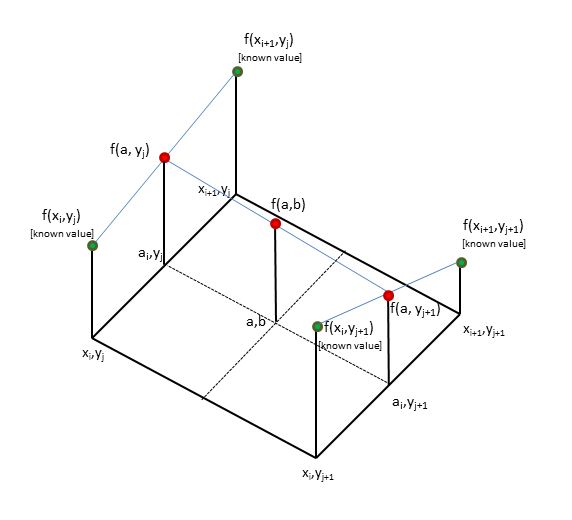
\includegraphics[width=0.7\textwidth]{interpolacion_bilineal.png}
    %
    \caption{Interpolación bilineal\protect\footnotemark}\label{fig:interp_bilineal}
    % \footnote{A}}
\end{figure}
\footnotetext{\url{https://stackoverflow.com/questions/8808996/bilinear-interpolation-to-enlarge-bitmap-images}}

\begin{figure}
    \centering
    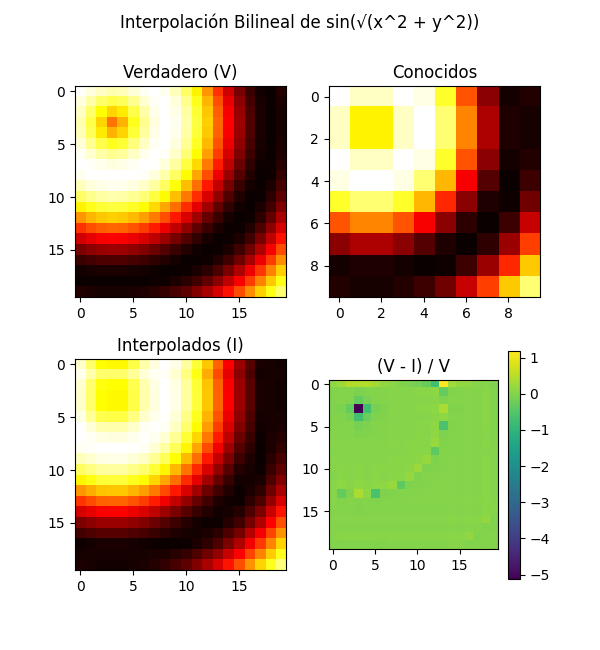
\includegraphics[width=0.6\textwidth]{bilineal.png}
    \caption{Interpolación bilineal de $\sin(\sqrt{x^2 + y^2})$}\label{fig:bilineal}
\end{figure}

La malla rectangular requerida para la interpolación bilineal del mapa de
$C_{D}$ se realizó a partir de los valores resultantes de las flujometrías con
\emph{OpenFOAM}~\parencite{openfoam}.
%
Debido al costo computacional que requieren las flujometrías, solo una cantidad
reducida de puntos se obtendrá con este método.
%
Se tiene como punto de partida una malla no rectangular, por lo que se utiliza
un método intermedio para obtener una matriz de puntos que pueda ser leída por
la interpolación bilineal.

Se probaron dos métodos para realizar esta interpolación, el método del punto más
cercano (MC) y la interpolación por la suma de la inversa de la distancia o IDW por
sus siglas en inglés (\emph{Inverse Distance Weighting}).
%
Estos se combinan con métodos de suavizado de promedio móvil con los $S$ valores
más cercanos.
%
Con este método cada valor original de la matriz se reemplaza por el promedio
aritmético de los valores a una distancia $S$ de cada celda evaluada.
%
En la Figura~\ref{fig:suavizado_promedio} se muestra este proceso para una
matriz de $5\times5$.

\begin{figure}[h!]
    \centering
    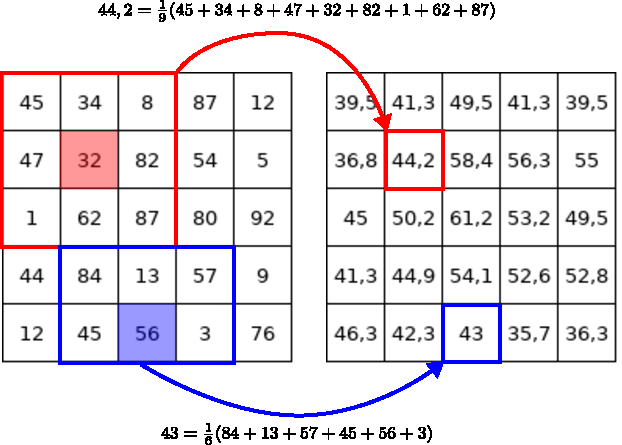
\includegraphics[]{/mapa_cd/suavizado.pdf}
    \caption{Suavizado por promedio con celdas vecinas, S=1}\label{fig:suavizado_promedio}
\end{figure}


El método del punto más cercano consiste en asignar para cada par $(x, y)$ el
valor conocido más cercano, ver Algoritmo~\ref{algo:mas_cercano}.

\begin{algorithm}
 \caption{Interpolación por punto más cercano}\label{algo:mas_cercano}
    \KwIn{\\
        $V_x, V_y$: valores de $x, y$ en los que se conoce el valor en $z$.\\
        $V_z$: valores conocidos de $z$.\\
        $I_x$: $n$ puntos de $x$ donde se quiere interpolar\\
        $I_y$: $m$ puntos de $y$ donde se quiere interpolar\\
        }

    \KwResult{Devuelve una matriz $I_{[n,m]}$ con los valores interpolados,
      donde a cada punto $I(x,y)$ se le asigna al valor de $v_z$ más cercano
      conocido. Da como resultado superficies escalonadas.}

    \BlankLine
     $I=zeros_{[n,m]}$\;
     \For{$i \gets 0$\KwTo$n$}{
        \For{$j \gets 0$\KwTo$m$}{
          $d = \sqrt{{(V_x - I_{xi})}^2 + {(V_y - I_{yj})}^2}$\;
            $I[i,j] = v_z[\min(d)]$\;
        }
     }
\end{algorithm}

La interpolación por IDW consiste en asignar a cada punto el resultado de un
promedio de los valores cercanos, ponderado por la distancia elevado a un
exponente arbitrario $p$.
%
Cuanto más grande el valor de $p$, más sensible es el método a los valores
cercanos.
%
La ecuación del promedio es la~(\ref{eq:idw}) y en el Algoritmo~\ref{algo:IDW}
se presenta el esquema utilizado.
%

\begin{equation} \label{eq:idw}
    f_p = \frac{\sum_{i=1}^{n} \frac{z_i}{d_i^p}} {\sum_{i=1}^{n}
    \frac{1}{d_i^p}}
\end{equation}

En la Figura~\ref{fig:mapas_interpolados} se muestra una comparación de ambos
métodos, para una malla de $C_{D}=f(\Delta P, l_{v})$ generada al azar.

\begin{algorithm}
    \caption{Interpolación IDW}\label{algo:IDW}
    \KwIn{\\
        $V_x, V_y$: valores de $x, y$ en los que se conoce el valor en $z$.\\
        $V_z$: valores conocidos de $z$.\\
        $I_x$: $n$ puntos de $x$ donde se quiere interpolar\\
        $I_y$: $m$ puntos de $y$ donde se quiere interpolar\\
        $p$: potencia a la que se eleva cada peso\\
        }

    \KwResult{Interpolación ponderada por inverso de la distancia. Dependiendo
      del valor de $p$, se obtienen valores más o menos suavizados.}

    \BlankLine
    $I=zeros_{[n,m]}$\;
    \For{$i \gets 0$\KwTo$n$}{
        \For{$j$\gets 0 \KwTo$m$}{
          $d = {\left[{(V_x - I_{xi})}^2 +{(V_y - I_{yj})}^2\right]}^{\frac{p}{2}}$\;
          \eIf{$\exists i : d[i] = 0$}{
            $I[i, j] = V_z[i]$\;
          }{
            $I[i,j] = \frac{\sum{V_{zi}/d_i}}{\sum \frac{1}{d}}$\;
          }
        }
     }
\end{algorithm}

% TODO:
% Modificar esto para mostrar la comparación entre métodos de interpolación con
% una función más convencional, como la que se ve en estas páginas:

% http://matlab.izmiran.ru/help/techdoc/math/poly_interp16.html
% https://medium.com/productive-data-science/how-to-interpolate-data-with-scipy-d314143285bc
% https://www.alglib.net/inverse-distance-weighting/
% https://www.mathworks.com/help/matlab/ref/peaks.html (peaks function)

\begin{figure}
    \centering
    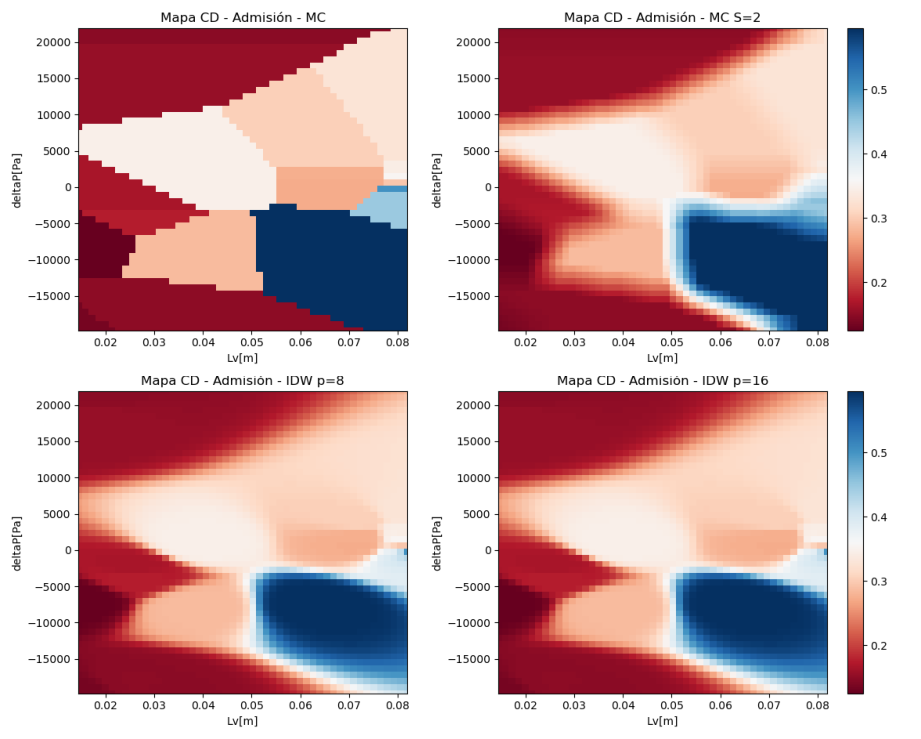
\includegraphics[width=.7\textwidth]{mapa_cd/mapa_cd.pdf}
    \caption{Comparación de métodos de interpolación}\label{fig:mapas_interpolados}
\end{figure}

%%%%%%%%%%%%%%%%%%%%%%%%%%%%%%%%%%%%%%%%%%%%%%%%%%%%%%%%%%%%%%%%%%%%%%%%%%%%%%%

\subsection{Área de Referencia}
%
El área de referencia utilizada por ICESym es el área de
cortina~(ver Ec.~\ref{eq:area_cortina}) y se expresa en el código del programa como el
área efectiva $F_{V}=A_{R}\cdot C_{D}$.
%
Como se indicó en el apartado~\ref{sec:cap2_cd}, para el  MRCVC el área de
referencia es el área frontal del puerto expuesta a la cámara, calculada como la
altura de la ranura $h_{p}$ multiplicada por la distancia entre el borde del
puerto y la paleta que delimita la cámara, denominada como $l_{v}$.

Este valor se afecta por el coeficiente de descarga intermedio $C_{D,int}$, que
puede ser un valor fijo o el resultado de interpolar de un mapa de $C_D$ para un
valor de cuerda y $\Delta P$ dado, como se indica en la ecuación~(\ref{eq:fv}).

\begin{equation}\label{eq:fv}
    F_v = C_{D,int}\cdot h_{p}\cdot l_{v}
\end{equation}

Tanto al inicio como al cierre del puerto ocurre solape de cámaras, por lo que
en estos intervalos angulares hay un valor de $C_D$ para cada cámara.
%
Cada valor se calcula con el flujo másico que atraviesa las secciones de entrada
correspondientes y el área de puerto expuesta por cada cámara.

\subsection{Interfaz con Optimizador}
%
Para lograr ejecutar el simulador automáticamente, se creó una librería de
funciones capaz de tomar como dato de entrada un archivo de configuración que
incluye geometría, velocidades a ejecutar y cantidad de ciclos de simulación,
entre otros.

Para ejecutar una instancia de ICESym se puede utilizar la interfaz gráfica de
usuario (GUI) ó ejecutarlo por línea de comando desde una consola.
%
El simulador de motores se ejecuta como un archivo de Python {\tt>> python
main.py}, el cual contiene las instrucciones que lanzan la simulación del
motor con la configuración requerida.
%

ICESym requiere de un archivo de configuración con los datos de la simulación a
realizar, este archivo se organiza como sigue:

\begin{forest}
  [config.py
    [Atmospheres]
    [Junctions]
    [Simulator]
    [Cylinders
      [Combustion]
      [Fuel]
      [Inyection]
      [Valves]]
    [Tanks]
    [Tubes]
  ]
\end{forest}

\begin{itemize}
  \item {\tt Atmospheres}: contiene el estado de la atmósfera, que es condición de
contorno de la simulación: presión, densidad y velocidad inicial.
  \item {\tt Cylinders}: geometría y condiciones de contorno, estado inicial,
tipo de motor, como así también de las válvulas.
  \item {\tt Valves}: geometría, tipo de válvula, modelo de $C_{D}$, perfil de alzada y
datos de $C_{D}$ y tubo conexionado.
  \item {\tt Junctions}: contiene información de las uniones entre tubos.
  \item {\tt Simulator}: configuración de la simulación, velocidades a simular,
propiedades de gas, tipo de motor, directorios, entre otros.
  \item {\tt Tanks}: volumen, masa y temperatura de pared de tanques.
  \item {\tt Tubes}: geometría, cantidad de nodos y conexiones de los tubos.
\end{itemize}

Los elementos de configuración intervenidos por el optimizador son {\tt
Cylinders}, {\tt Valves}, {\tt Simulator} y {\tt Tubes}; donde se  modifican los
siguientes valores:

\begin{itemize}
  \item {\tt Simulator}:
        \begin{itemize}
          \item {\tt RPMS}: Velocidades a simular (por ejemplo una lista de [1000,
2000, \ldots, 9000).
          \item {\tt NCYCLES}: cantidad de ciclos por velocidad (un entero mayor o igual a 1).
          \item {\tt FOLDER NAME}: nombre de la carpeta donde se guardan los
resultados de la simulación.
          \item {\tt SHOW INFO}: selector para mostrar o no información de la simulación.
          \item {\tt CONFIG DATA}: archivo donde se guarda la configuración utilizada.
        \end{itemize}
  \item {\tt Cylinders} $\longrightarrow$ Valves
        \begin{itemize}
          \item {\tt LvI}: perfil de alzada del puerto de admisión.
          \item {\tt LvE}: perfil de alzada del puerto de escape.
          \item {\tt IPO}: ángulo de apertura del puerto de admisión.
          \item {\tt IPC}: ángulo de cierre del puerto de admisión.
          \item {\tt EPO}: ángulo de apertura del puerto de escape.
          \item {\tt EPC}: ángulo de cierre del puerto de escape.
          \item {\tt cd\_model}: selector de modelo de $C_{D}$.
                \begin{itemize}
                  \item $C_{D}l_{v}$ valores de alzada para el mapa de $C_{D}$(
para modelo de 2 variables).
                  \item $C_{D}d_{p}$ valores de $\Delta_{P}$ para el mapa de
$C_{D}$ (para modelo de 2 variables).
                  \item $C_{D}$ valores de $C_{D}$ relacionados con alzada (para modelo de 1 variable).
                \end{itemize}
          \item $D_{v}$: diámetro de la cabeza de la válvula.
        \end{itemize}
  \item Tubes
        \begin{itemize}
          \item longitud: longitud total del tubo de admisión o escape.
        \end{itemize}
\end{itemize}

%%%%%%%%%%%%%%%%%%%%%%%%%%%%%%%%%%%%%%%%%%%%%%%%%%%%%%%%%%%%%%%%%%%%%%%%%%%%%%%%
%%%%%%%%%%%%%%%%%%%%%%%%%%%%%%%%%%%%%%%%%%%%%%%%%%%%%%%%%%%%%%%%%%%%%%%%%%%%%%%%
%%%%%%%%%%%%%%%%%%%%%%%%%%%%%%%%%%%%%%%%%%%%%%%%%%%%%%%%%%%%%%%%%%%%%%%%%%%%%%%%


\section{Optimizador y Algoritmo Genético}
%
% Se seleccionó un algoritmo genético (AG) como método de optimización por ser un
% método sencillo de programar además, este tipo de algorimto es de utilidad
% cuando se tiene una solución con uno o más máximos óptimos locales ó cuando no
% se tiene certeza sobra la suavidad de la función a evaluar.
%

Se seleccionó un algoritmo genético (AG) para realizar la optimización de la
geometría del MRCVC por la simplicidad y facilidad de implementación del mismo.
%
Si bien este tipo de métodos no garantiza que se alcance un resultado óptimo,
en la práctica se ha observado que alcanzan soluciones muy cercanas a las
óptimas tras pocas iteraciones del método~\parencite{goldberg}\parencite{shi}.

Una de las ventajas de este método es que no requiere información del gradiente
de la función que se está evaluando, lo cual es útil cuando no se puede asegurar
la existencia de la derivada de la función en todo el dominio ó cuando se tiene
una función con más de un máximo o mínimo local.
%
Además, el punto de partida de la optimización es una población generada al
azar, se tiene un muestreo aleatorio del dominio que se está evaluando.
%
Esto hace que el método sea poco susceptible a dar como resultado óptimos
locales.

Se puede decir que un algoritmo genético es un método de búsqueda aleatoria
guiada.
%
¿Cómo difieren los AG de los métodos tradicionales de búsqueda?
%
\begin{enumerate}
  \item Los AG pueden operar sobre una representación de las variables estudiadas y
no necesariamente sobre las variables de estudio.
  \item Cada iteración utiliza un conjunto de datos con cierto grado de
aleatoriedad.
  \item Utilizan una función objetivo para evaluar cada punto sin necesidad de
conocer la derivada de la función que se está evaluando.
  \item Los AG usan reglas probabilísticas de decisión.
\end{enumerate}


% \subsection{Componentes básicos de un AG}
%
Los mecanismos básicos que hacen a un algoritmo genético son: 1) \emph{selección}, 2)
\emph{cruza} y 3) \emph{mutación}.
%
El funcionamiento básico se sintetiza en el Algoritmo~\ref{algo:genetico}.

La \emph{selección} consiste en crear individuos a partir del puntaje que devuelve
una función objetivo, la cual es la encargada de guiar el proceso de
optimización dando mayor o menor puntaje a un candidato según el resultado que
se quiere obtener.
%
Este paso significa que, aquellos individuos a los cuales se les asignó un
puntaje más elevado tienen más probabilidades de ser copiados o de
``transmitir'' sus parámetros a la iteración siguiente.
%
Este proceso imita en cierta forma la selección natural o evolución Darwiniana y
de aquí viene el nombre de algoritmo genético o evolutivo.

El segundo operador es la \emph{cruza}, que consiste en combinar los parámetros
de dos individuos para obtener uno nuevo, esto se asemeja a la reproducción.

Finalmente la \emph{mutación} es la encargada de modificar aleatoriamente uno o más
parámetros de cada nuevo individuo.
%
Este operador juega un rol secundario pero muy importante en la simulación.
%
Es secundario porque se pueden alcanzar soluciones satisfactorias sin que
aplique este operador en la población.
%
Es importante porque utilizando probabilidades pequeñas de ocurrencia (de la
mutación), permite evitar la pérdida temprana de información relevante por
convergencia temprana de la simulación.
%
Por otro lado, en caso de que la probabilidad de mutación sea muy alta, el AG se
convierte en un método de búsqueda aleatoria.

\begin{algorithm} \caption{Algoritmo de optimización}\label{algo:genetico}
  Inicializar población, al azar o a partir de una población ``semilla''.\;
  %
  \While{no se cumpla condición de parada}{
    %
    \emph{Seleccionar} a los individuos más aptos, evaluándolos según la función objetivo.\;
    %
    \emph{Cruzar} los candidatos seleccionados para crear la nueva población (la
próxima iteración del método)\;
    %
    \emph{Mutar} algunos individuos de la nueva población\;
    %
    \If{se cumple la condición de parada}{
      Parar\;
    }
  }
  {Guardar resultados\;}
\end{algorithm}

Gran parte de este trabajo consistió en adaptar el uso de ICESym y emplearlo
como base para generar una función objetivo, aprovechando la cualidad de ``caja
negra'' con la que se puede implementar el simulador.
%
Para lograr esto se modificó parte del código de ICESym con el objetivo de
facilitar la configuración, ejecución y lectura de los resultados que arroja el
simulador y así poder ejecutar de manera automática una simulación con una
configuración particular del motor.
%
Otro aspecto del optimizador que se desarrolló, es el de poder ejecutar
múltiples instancias de ICESym en paralelo con el fin de reducir el tiempo de
ejecución de cada generación, pudiendo evaluar varios motores (o individuos) al
mismo tiempo.

Para la primera iteración se programaron desde cero los algoritmos y funciones
necesarias para llevar a cabo la optimización con el AG.
%
Posteriormente se tomó la librería DEAP~\parencite{DEAP_JMLR2012} y se
modificaron los operadores a medida, para poder utilizarlos con ICESym.

En los apartados siguientes se describe la implementación de cada uno de los
operadores en el optimizador.

\subsection{Población}
%
Se decidió representar cada motor como un vector con las dimensiones y reglaje
que definen la geometría del sistema de intercambio de gases, los cuales se
listan en la Tabla~\ref{tab:param_motor}.
%
Se limitaron los valores que puede tomar cada parámetro para que la geometría
resultante se asemeje a la geometría del motor utilizado en trabajos anteriores,
aprovechando así los resultados obtenidos en el primer barrido paramétrico.

\begin{table}[h!]
  \centering
  \begin{tabular}{rllll} \toprule
    Nº & Parámetro & Descripción & Sistema & Límites \\ \midrule
    1 & DTA & Diámetro de tubo & Admisión & [60, 100] mm \\
    2 & DTE & Diámetro de tubo & Escape & [60, 100] mm\\
    3 & LIT & Largo de tubo & Admisión & [300, 2000] mm\\
    4 & LET & Largo de tubo & Escape & [300, 2000] mm\\
    5 & IIA & Ángulo geométrico de apertura & Admisión & [0,90]º \\
    6 & IFA & Ángulo geométrico de cierre & Admisión & [IIA, 90]º \\
    7 & IIE & Ángulo geométrico de apertura & Escape & [0, 90]º \\
    8 & IFE & Ángulo geométrico de cierre & Escape & [IIE, 90]º \\ \bottomrule
  \end{tabular}
  \caption{Parámetros que representan al motor}\label{tab:param_motor}
\end{table}

Los vectores que hacen a cada motor se representan como un número binario de 40
dígitos, ocupando 5 dígitos para representar cada uno de los 8 parámetros que
hacen a cada motor.
%
Esto facilita la implementación de los operadores de selección, cruza y
mutación, pudiendo aprovechar implementaciones de operadores existentes en
librerías como DEAP.
%
Estos 8 números binarios luego se convierten en una lista de enteros mediante
una transformación lineal $f(x)=a\cdot x+b$, en la que se ingresa con un entero
entre 0 y $2^{n}-1$ para ir del número binario a un decimal, siendo $n$ la
cantidad de dígitos del número binario (en este caso 5).
%
Los coeficientes $a$ y $b$ son tales que $f(0)=x_{0}$ y $f(2^{n}-1) = x_{1}$,
donde $x_{0}$ y $x_{1}$ son los extremos del rango para el que se quiere aplicar
la transformación.
%
Estos coeficientes ($a$ y $b$) son particulares a cada parámetro, porque se
determinan de acuerdo a los valores que puede tomar cada uno.

De este modo se obtiene el valor de cada uno de los parámetros que hacen a la
configuración particular de cada motor en ICESym.
%
El orden de los mismos se mantiene constante, por lo que cada sección del número
representa una característica en particular del motor.

A modo de ejemplo, en la Figura~\ref{fig:pop_bit} se muestra un número generado
aleatoriamente, la transformada para los primeros 5 dígitos que corresponden al
diámetro del tubo de admisión, 001111.
%
Si se desea que el diámetro del tubo de admisión varíe entre 60 y 100 mm, se
deben obtener los coeficientes $a$ y $b$ para la transformación lineal  a partir
del largo del número binario que se va a utilizar, {\tt{binLen}}, y los valores
mínimos y máximos del rango sobre el que se quiere transformar el valor de
entrada: $vMin=60$ y $vMax=100$.

Los coeficientes $a$ y $b$ se obtienen a partir de:
\begin{align*}
  a &= \frac{vMax-vMin}{2^{binLen} - 1} =\frac{100-60}{2^{5}-1} = 1,2903\\
  b &= vMin=60
\end{align*}

Luego, el número binario transformado a entero vale:
\begin{equation*}
  00111 \longrightarrow 0\cdot 2^{4} + 0\cdot 2^{3} + 1\cdot 2^{2} + 1\cdot 2^{1} + 1\cdot 2^{0} = 7
\end{equation*}

Finalmente, con los coeficientes ($a$, $b$) y el binario transformado en entero,
se tiene que DTA vale

\begin{equation*}
  DTA = a\cdot x + b = (1,2903\cdot 7 + 60) = 69 mm = 0,069 m
\end{equation*}


\begin{figure}[h!]
  \centering
  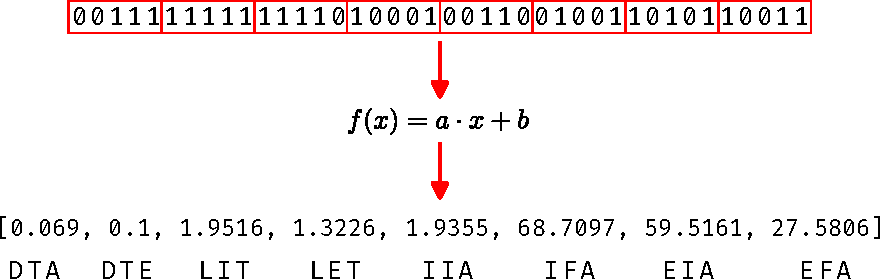
\includegraphics[]{genetico/map_to_engine.pdf}
  \caption{Representación del individuo}\label{fig:pop_bit}
\end{figure}


\subsection{Selección}

Para crear la nueva población se debe elegir a los nuevos candidatos basándose
en los puntajes de la población actual.
%
Hay varios métodos diferentes de selección, como lo son de ruleta, aleatoria,
por puntaje y de tipo torneo.
%
Para este trabajo se seleccionó el método de torneo, es uno de los métodos más
populares para los procesos de selección de AG.

El método consiste en seleccionar $k$ individuos de la población al azar, se
comparan los puntajes de estos individuos y resulta ``ganador'' aquel que tenga
más puntaje.
%
El proceso se repite $N$ veces hasta generar la nueva población.

El parámetro $k$ es el tamaño de torneo y comúnmente se utiliza
2~\parencite{oladele}.
%
A mayores valores para $k$ se tiene una mayor pérdida de diversidad en los
resultados\parencite{blickle} porque reduce la posibilidad de que candidatos con
menor puntaje sean seleccionados para la nueva generación (convergencia
temprana).

Para este torneo se utilizó además un \emph{salón de la
  fama}~\parencite{wirsansky} de 1 individuo.
%
Esto significa que el mejor individuo de la población actual es automáticamente
seleccionado para la iteración siguiente y la selección por torneo se realiza
$N-1$ veces.

\subsection{Cruza}
%
El operador de cruza se encarga de combinar los genes  de dos individuos para
producir uno nuevo.
%
Se encarga de combinar/intercambiar los parámetros de los individuos
``cruzados'' para generar uno nuevo.
%
Para individuos representados por un vector se suelen usar operadores de tipo
cruza de uno o múltiples puntos, también se utilizan mecanismos de cruza
uniforme.
%
El método seleccionado es \emph{cruza de dos puntos}.
%
En este método se corta el vector que forma al individuo en dos puntos, la
posición de estos puntos se selecciona al azar, manteniendo el largo original de
los vectores.
%
Los individuos ``cruzados'' se combinan de forma complementaria como se indica
en la Figura~\ref{fig:cr2puntos}, el algoritmo~\ref{algo:cr2puntos} esquematiza
el proceso.

\begin{figure}[h!]
  \centering
  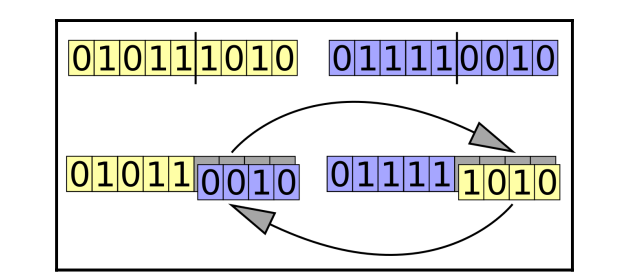
\includegraphics[width=0.5\textwidth]{cruza2puntos.png}
  \caption{Cruza de dos puntos~\parencite{wirsansky}}\label{fig:cr2puntos}
\end{figure}


\begin{algorithm}[h!]
  \KwIn{\\
    $ind_{1}, ind_{2}$: dos individuos de entrada, por ej. [101\ldots011], [110\ldots100].\\
    EA(a, b): devuelve un entero al azar entre los enteros a y b.\\
    L(a): devuelve la cantidad de elementos en a.}
  \KwOut{\\
    $ind_{1}, ind_{2}$: individuos de entrada modificados}
  \SetKwFunction{EA}{EA}
  \SetKwFunction{L}{L}
  % \SetKwFunction{min}{min}
  \BlankLine
  s = min(\L{$ind_{1}$}, \L {$ind_{2}$})\;
  $CX_{1} = \EA{1, s}$\;
  $CX_{2} = \EA{1, s-1}$\;
  \eIf{$CX_{1} \geq CX_{2}$}{
    $CX_{2} = CX_{2}+1$\;
  }{
    $aux=CX_{1}$\;
    $CX_{1}=CX_{2}$\;
    $CX_{2}=aux$\;
  }
  $aux = ind_{1}$\;
  $ind_{1}[CX_{1}:CX_{2}] = ind_{2}[CX_{1}:CX_{2}]$\;
  $ind_{2}[CX_{1}:CX_{2}] = aux[CX_{1}:CX_{2}]$\;
  \Return{$ind_{1}, ind_{2}$}\;
  \caption{Cruza de dos puntos}\label{algo:cr2puntos}
\end{algorithm}

\subsection{Mutación}
%
La mutación juega un rol secundario pero importante en los AG, consiste en
modificar aleatoriamente alguno de los parámetros que definen a un individuo.
%
Este mecanismo contribuye a la diversidad de soluciones y por ende reduce la posibilidad de
convergencia temprana.
%
Se utilizan probabilidades bajas de mutación, en el caso extremo si la
probabilidad de mutación es del $100\%$ el AG se convierte en un método de
búsqueda aleatoria.
%
Algunos de los métodos de mutación utilizados son:

\begin{enumerate}
  \item Flip Bit
  \item Intercambio
  \item Inversión
  \item Reordenado Aleatorio
\end{enumerate}

En este trabajo se utiliza el método de reordenado aleatorio en el cual se
modifica al azar el orden de los números que hacen al individuo, modificando los
índices de la lista que define el arreglo, por ejemplo: $11100 \rightarrow 10011$.
%
El pseudocódigo de este proceso se presenta en el algoritmo~\ref{algo:flipbit}.

\begin{algorithm}
  \caption{Flip Bit}\label{algo:flipbit}
  \DontPrintSemicolon
  \KwIn{
    $A = (a_{1}, a_{2}, \ldots, a_{n})$ es un vector compuesto de unos y ceros.\\
    $R$, es una función aleatoria que devuelve un número real entre 0 y 1.\\
    $p$, es un número real entre 0 y 1 que representa la probabilidad de mutación.
  }

  \For{i=1 \KwTo n}{
    \If{$R < p$}{
      \lIf{$A_{i}=1$}{$A_{i}=0$}
      \lElse{$A_{i}=1$}
      }
  }
    \Return A\;
\end{algorithm}

\subsection{Función Objetivo}\label{sec:funcion_objetivo}
%
La función objetivo es la encargada de dar puntaje a los individuos, en la
analogía con la selección natural esta función es el ambiente.
%
Determina la aptitud de un motor con respecto a otro en lo que respecta a
\emph{performance} del sistema de intercambio de gases.
%
Inicialmente se propuso que la función objetivo sea la suma de los rendimientos
volumétricos a todas las velocidades simuladas $s=\sum \eta_{v}$.
%
Este tipo de funciones dió como resultado una curva de $\eta_{v}$ aserrada como
se muestra en la Figura~\ref{fig:curva_aserrada}.

\begin{figure}[h!]
  \centering
  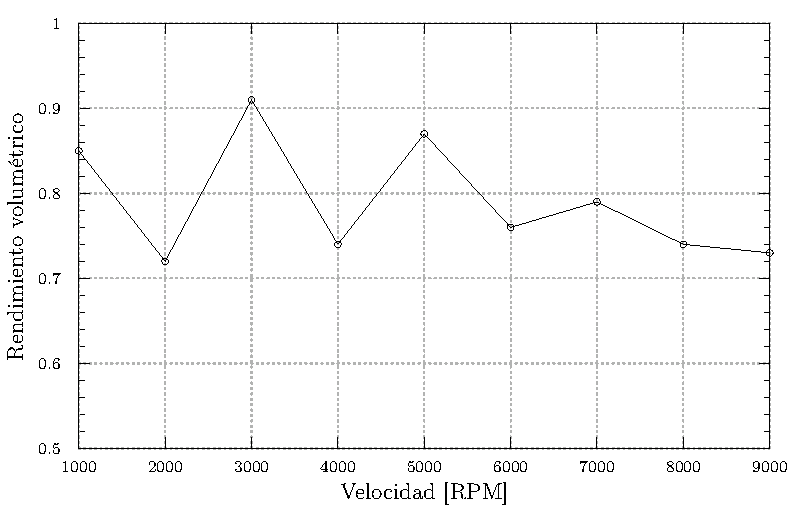
\includegraphics[width=0.7\textwidth]{gnuplot/rendimiento_aserrado.pdf}
  \caption{Curvas de rendimiento volumétrico aserradas}\label{fig:curva_aserrada}
\end{figure}

Esta curva aserrada es poco deseable porque significa una entrega de torque y
potencia dispar, por este motivo se modificó la función objetivo para favorecer
curvas suaves y preferentemente con un solo punto de inflexión.
%
Se implementó una suma ponderada para obtener un rendimiento volumétrico máximo
en un valor cercano a 6000 RPM de modo de aprovechar las características de
balanceo de fuerzas y mayores velocidades de giro de los motores rotativos.
%
La aptitud resulta de la suma del rendimiento volumétrico y el inverso de la
fracción de gases residuales, lo cual probó ser la función objetivo que mejores
resultados dió.
%p
La metodología utilizada se resume a continuación.

\begin{enumerate}
        \item Se evalúa cada motor, calculando el rendimiento volumétrico
$\eta_{v}$ y la fracción de gases residuales $x_{r}$ para cada velocidad de giro
simulada.
        \item Con $\eta_{v} = (\eta_{v,1}, \ldots ,\eta_{v,n})$ y
$x_{r}=(x_{r,1},\ldots,x_{r,n})$ se realiza la siguiente suma para cada velocidad
$S_{i}=\eta_{v,i} + x_{r,i}^{-1}$.
        \item Cada motor tiene un vector o lista de valores
$S = (S_{1},\ldots,S_{n})$ para cada velocidad evaluada, con la cual se calcula
el puntaje del motor como:
        \begin{equation}
        f = \sum_{i=1}^{n}{S_{i}} + S_{k}^{2}
      \end{equation}

El valor $S_{k}$ es el puntaje para la $k$-\textit{ésima} velocidad de giro (6000 RPM en
este caso) y se eleva al cuadrado para favorecer altos rendimientos en esta
velocidad.
\end{enumerate}


Durante las primeras iteraciones del método hay una gran cantidad de geometrías
inválidas que devuelven puntaje muy bajo o nulo.
%
En caso de que alguna de las soluciones tenga un puntaje relativamente alto,
existe la posibilidad de una dominancia temprana de la población, provocando
una convergencia temprana de la optimización.
%
Estos candidatos tienen una mayor probabilidad de ``pasar'' sus características
geométricas a las iteraciones siguientes y es algo especialmente problemático en
optimizaciones con poblaciones de alrededor de 100 individuos.

Para reducir la posibilidad de una convergencia temprana se utiliza un método de
escalado de puntajes, que consiste en una transformación lineal en la que se
define el puntaje bruto de un individuo como $f$ y el puntaje escalado como
$f'$, la relación entre ambos es $f' = a\cdot f + b$.
%
Los coeficientes $a$ y $b$ se determinan de modo que $f'_{media}=f_{media}$, de
este modo un motor con puntaje promedio tiene la misma influencia sobre la
población ya sea con la aptitud original o escalada.
%
Para controlar la influencia del mejor individuo de una generación sobre la
próxima, los puntajes se transforman de tal modo que
$f'_{max}=C_{mult}f_{media}$.
%
El valor de $C_{mult}$ es la cantidad de copias que se espera obtener del mejor
de los candidatos en la generación siguiente y se usa en $1,2$ a $2$ para
poblaciones de entre 50 y 100 individuos~\parencite{goldberg}.

Hacia el final donde la diferencia entre puntajes de los individuos de la
población tiende a achicarse, el parámetro $C_{mult}$ cumple la función de
acrecentar las diferencias entre individuos.

En caso de existir individuos con puntaje muy bajo o nulo se hace un
pre-escalado del puntaje que fija el mínimo en $f'_{min}=0$.
%
El procedimiento se lista en los algoritmos \ref{algo:pre-escala} y
\ref{algo:pop_scale}.


\begin{algorithm} \caption{Algoritmo de pre-escalado}\label{algo:pre-escala}
  \KwIn{\\
    $F$, es un vector que contiene los puntajes de todos los individuos\;\\
    $C_{mult}$, es un multiplicador para el escalado, se suele usar
$C_{mult}\in[1.2, 2]$\;\\ }
  \KwOut{\\
    $a, b$, son los coeficientes para la transformación lineal $f(x)=a\cdot x + b$\;
  }
  \SetKwFunction{max}{max}
  \SetKwFunction{min}{min}
  \SetKwFunction{media}{media}
  \BlankLine

  $u_{max} = \max{F}$\;
  $u_{min} = \min{F}$\;
  $u_{medio} = \media{F}$\;
  \eIf{$u_{min}> aux = (C_{mult}\cdot u_{medio} - u_{max}) \mathbin{/} (C_{mult}-1)$
    }{
    $\Delta_{u} = u_{max}-u_{avg}$\;
    $a = (C_{mult} - 1) \cdot u_{avg} / \Delta u$\;
    $b = u_{avg} \cdot (u_{max} - C_{mult} \cdot u_{avg}) \Delta_{u} $\;
  }{
    \eIf{$\Delta \neq 0$}{
      $a = u_{avg} \mathbin{/} \Delta_{u}$\;
      $b = -u_{min} \cdot u_{avg} \mathbin{/} \Delta_{u}$ \;
    }{
      $a=1$\;
      $b=0$\;
    }
  }
  \Return{$a, b$}
\end{algorithm}


\begin{algorithm}\caption{Escalado de población}\label{algo:pop_scale}
  \KwIn{\\
    $f$, es la aptitud.\\
    $a, b$, son los parámetros de la función de pre-escalado. \\
  }
  \KwOut{\\
  $f^{*}$, los puntajes escalados.}
  \SetKwFunction{ps}{PreEscalado}
  \SetKwFunction{ll}{Largo}
  \SetKwFunction{esc}{Escala}
  \BlankLine

  $a, b = \ps{f, 2}$\;
  $f^{*} = ()$ \;
  $n = \ll{f}$\;
  \For{$i=1$ \KwTo $n$}{
    $f^{*}_{i} = a\cdot f_{i} + b$\;
  }
  \Return{$f^{*}$}\;
\end{algorithm}

% Con la población definida se procede a los evaluar cada motor con la función
% objetivo, la cual se definió de manera tal de favorecer curvas de rendimiento
% volumétrico suaves y valores altos a mayores RPM.\@

% La suavidad de la curva de rendimiento volumétrico se calcula midiendo los
% cambios de pendiente de la derivada la cual se aproxima con la fórmula de
% diferencia progresiva~\ref{eq:derivada}.
% %
% Solamente interesa el signo, por lo que el valor de $h$ en el denominador no
% interesa y se hace 1, con esto la función objetivo queda como el
% algoritmo~\ref{alg:funcObj}.

% \begin{equation}\label{eq:derivada}
%   f' = \frac{f(i+1) - u(i)}{h}
% \end{equation}

% Una vez evaluados todos los motores de la población, se debe seleccionar los
% individuos que formarán la siguiente iteración del algoritmo.
% %
% El método de selección es de tipo TORNEO, en el cual se seleccionan los mejores
% $k$ individuos de un grupo al azar de $N$ candidatos.
% %

% Con los nuevos candidatos seleccionados, se procede a variar la población,
% realizando la cruza y mutación.

% Luego se toman pares de individuos y de acuerdo a la probabilidad de cruza, se
% combinan con el método seleccionado.

% Finalmente se realiza una segunda iteración sobre la nueva población, aplicando
% el método de mutación a cada individuo, de acuerdo a la probabilidad de
% mutación indicada.
%

%%%%%%%%%%%%%%%%%%%%%%%%%%%%%%%%%%%%%%%%%%%%%%%%%%%%%%%%%%%%%%%%%%%%%%%%%%%%%%%%
%%%%%%%%%%%%%%%%%%%%%%%%%%%%%%%%%%%%%%%%%%%%%%%%%%%%%%%%%%%%%%%%%%%%%%%%%%%%%%%%
%%%%%%%%%%%%%%%%%%%%%%%%%%%%%%%%%%%%%%%%%%%%%%%%%%%%%%%%%%%%%%%%%%%%%%%%%%%%%%%%

\section{OpenFOAM}\label{sec:3_openfoam}
%
Las flujometrías se realizaron con \emph{OpenFOAM}, un software de
Fluidodinámica Computacional, o CFD por sus siglas en inglés, de código libre y
abierto e

scrito en ``C++''.
%
% La herramienta seleccionada para realizar las flujometrías es OpenFOAM, por ser
% una herramienta libre y de código abierto.
%
Junto con este programa se utilizaron otras herramientas libres para generar la
geometría a modelar y post-procesar los resultados..
%
El esquema de trabajo para realizar las simulaciones consistió en:

\begin{enumerate}
        %
    \item Pre-procesado
      %

        \begin{enumerate}
                %
            \item Definir la geometría a analizar.
              %

          \item Generar una malla con un tamaño de elemento adecuado (la
solución a problemas de CFD depende fuertemente de la cantidad y tamaño de
celdas utilizadas).
              %
            \item Seleccionar los modelos adecuados.
              %
            \item Definir las propiedades del fluido.
              %
            \item Definir las condiciones de borde.

              %
        \end{enumerate}
        %
    \item Solver
      %
    \begin{enumerate} \item Seleccionar el solver a utilizar.
            %
            \item Ejecutar la simulación.
            %
    \end{enumerate}
        %
\item Post-procesado
      %
    \begin{enumerate}
                %
        \item Visualizar los resultados de las distintas variables de la
            simulación.
            %
        \item Extraer la información necesaria.
            %
    \end{enumerate}
        %
\end{enumerate}

%%%%%%%%%%%%%%%%%%%%%%%%%%%%%%%%%%%%%%%%%%%%%%%%%%%%%%%%%%%%%%%%%%%%%%%%%%%%%%%%

\section{Esquemas de Discretización}

Se utilizan para resolver ecuaciones de variables continuas con funciones
discretas en tiempo y espacio.
%
Se deben seleccionar esquemas para resolver:

\begin{itemize}
  \item Primera derivada temporal
  \item Interpolación
  \item Gradiente
  \item Divergencia
  \item Gradientes normales a superficies
  \item Laplacianos
\end{itemize}


\subsection{Derivadas temporales, $\delta / \delta t$}
%
Estas derivadas se discretizan con el método de Euler\parencite{burden}, que
aproxima la integración de un paso $n$ a $n+1$ con $y_{n+1}-y_{n}\simeq hf_{n}$
donde $h = t_{n+1}-t_{n}$ es el paso temporal y $f_{n}=f(t_{n},y_{n})$.
%
Para el esquema de Euler hacia atrás la aproximación es
$y_{n+1}-y_{n}\simeq h f_{n+1}$.
%
A este esquema se le agrega un coeficiente $\gamma\in[0,1]$ de modo que:

\begin{equation}
  y_{n+1}-y_{n} \simeq \gamma h f_{n+q} + (1-\gamma)h f_{n}
\end{equation}

Con $\gamma=1/2$ el esquema es equivalente a Crank-Nicolson estándar.
%
Se puede convertir al esquema de Euler hacia adelante con $\gamma=0$.

\subsection{Gradientes}
%
Se discretiza utilizando integración Gaussiana con interpolación lineal entre
valores de celdas.
%
El método define al gradiente medio en un elemento de volumen finito con
centroide \textbf{C} y volumen $V_{c}$ en términos de los flujos a través de sus
caras, como lo indica la ecuación~(\ref{eq:green_gauss_gradient}).
%
Para esto se requiere conocer los valores de la variable $\phi_{f}$ en las caras
vecinas e información del área de la celda y su normal $(\vec{S}_{f})$.

\begin{equation}
  \label{eq:green_gauss_gradient}
  \nabla \phi_{P} = \frac{1}{V_{c}}\sum_{f} \vec{S}_{f}\phi_{f}
\end{equation}

El método de volúmenes finitos utiliza valores en las caras de las celdas, por
lo que se debe aproximar el valor de la variable en una cara dada para obtener
el valor del gradiente en dicha celda.
%
Los valores de $\phi_{f}$ se obtienen de una interpolación lineal entre valores
conocidos de celdas adyacentes.
%
Un método de interpolación entre celdas puede ser:

\begin{align}
  \label{eq:interpolacion_lineal_caras}
  \alpha &= \frac{|{\vec{r}_{N}-\vec{r}_{f}}|} {|{\vec{r}_{N}-\vec{r}_{P}}|}\\
  \phi_{f} &= \alpha\phi_{P}+(1-\alpha)\phi_{N}
\end{align}

Donde $\alpha$ es un factor de ponderación geométrico entre las celdas
\textbf{P}, \textbf{N} y $\vec{r}$ es el vector posición del centroide de las
celdas.

La interpolación se puede limitar para que los valores obtenidos se encuentren
entre el mínimo y máximo de las celdas vecinas, este método se denomina
``limitado''.

\subsection{Gradiente normal a una superficie}
%
Este gradiente es evaluado en la cara de la celda.
%
Es la componente (normal a la cara) del gradiente entre los valores de los
centroides de 2 celdas conectadas por la cara evaluada.
%
En general las mallas utilizadas para modelar geometrías reales no son
ortogonales.
%
Esto implica que el vector $\vec{CF}$ que une el centroide de dos celdas
contiguas (\textbf{C} y \textbf{F}) no necesariamente es colineal con el vector
$\vec{S_{f}}$ normal a la superficie.
%
El gradiente  evaluado en la cara de una celda $(\nabla\cdot\vec{e})_{f}$, en la
dirección del vector unitario que une los centroides de C y F ($\vec{e}$), se
puede expresar como se indica en la Ecuación~\ref{eq:gradiente_normal}

\begin{align}
    \label{eq:gradiente_normal}
  \vec{e} &= \frac{\vec{r}_{F}-\vec{r}_{C}}{||\vec{r}_{F}-\vec{r}_{C}||} = \frac{\vec{d}_{CF}}{d_{CF}} \\
  (\nabla \phi \cdot \vec{e})_{f} &= \frac{\partial \phi}{\partial n} = \frac{\phi_{F} - \phi_{C}}{||\vec{r_{C}}-\vec{r_{F}}||} = \frac{\phi_{F} - \phi_{C}}{d_{CF}}
\end{align}

Donde el subíndice $f$ indica que se evalúa en la cara de una celda.
%
El vector de superficie $\vec{S_{f}}$ se puede escribir en términos de sus
componentes normal y tangente a la cara $f$ en la que es evaluado:

\begin{equation}
    \vec{S_{f}}= \vec{E_{f}} + \vec{T_{f}}
\end{equation}

De esta forma, el gradiente de la variable $\phi$ en mallas no ortogonales se
puede expresar en términos de las componentes normal y tangente a la cara de la
celda~\parencite{moukalled}.
%
El término \textbf{E} indica la componente del gradiente normal a la cara y
\textbf{T} la componente tangente.

\begin{align}
\label{eq
}
%
{(\nabla \phi)}{f}\cdot \vec{S{f}} &= {(\nabla \phi)}{f}\cdot \vec{E{f}} + {(\nabla \phi)}{f}\cdot \vec{T{f}} \
%
&= \vec{E_{f}}\frac{\phi_{F}-\phi_{C}}{d_{CF}}+ {(\nabla \phi)}{f}\cdot \vec{T{f}}
\end{align}

%
Algunos esquemas de discretización de este tipo de gradientes son:
\begin{itemize}
\item No corregido
\item Ortogonal
\item Corregido y limitado
\end{itemize}

La corrección ortogonal ajusta el vector $\vec{d_{CF}}$ para que sea colineal con el vector $\vec{S_{f}}$, asegurando que el cálculo del gradiente se haga en la dirección normal a la superficie.
%
La corrección limitada aplica la corrección ortogonal, sumando un término adicional para tener en cuenta la desviación entre $\vec{d_{CF}}$ y $\vec{S_{f}}$ debido a la no ortogonalidad, generalmente en términos de $\cos^{-1}{\theta}$, donde $\theta$ es el ángulo entre el vector normal a la cara y el vector $\vec{d_{CF}}$.

% Divergencia
\subsection{Divergencia}
%
Se utiliza un esquema de integración Gaussiana con interpolación lineal para
la discretización de la divergencia.

Dependiendo de los tipos de variable, se utilizan diferentes esquemas de
interpolación disponibles son:
%
\begin{itemize}
        \item centrada
        \item hacia adelante
        \item hacia atrás
        \item limitada
\end{itemize}

\subsection{Laplacianos}
%
Los términos Laplacianos se discretizan utilizando integración Gaussiana con
interpolación lineal.
